\documentclass[twoside,12pt]{article}
%\usepackage{amsmath,amsfonts,amsthm,fullpage}
%\usepackage{mymath}
%\usepackage{algorithm}
%\usepackage{algorithmic}
\usepackage{graphicx}
\newcommand{\imsize}{0.5\linewidth}

\begin{document}

\title{CS 8803 DL Assigment 2}
\author{Jingdao Chen}
\date{Feb 24}
\maketitle
\openup 1em

\section{Optimization}

The plots of training and test error for each method is shown below:

\subsection{Stochastic Gradient Descent}

Learning rate = 1e-3

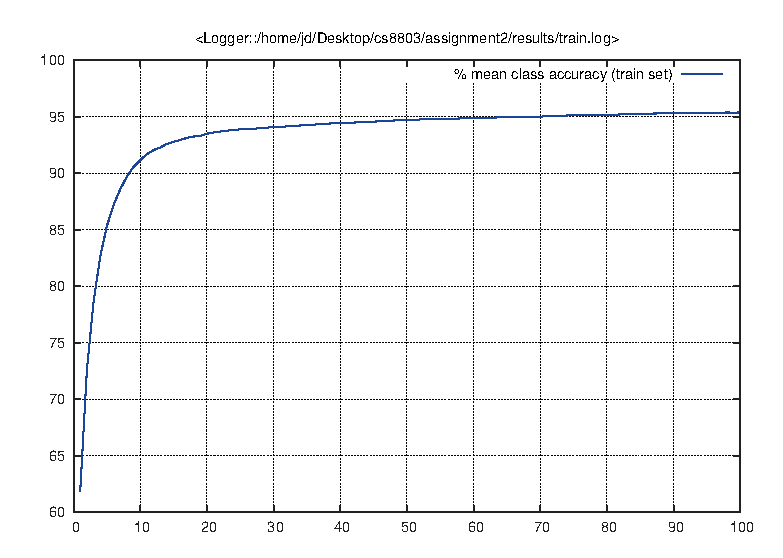
\includegraphics[width=\imsize]{assignment2/results/sgd_train}
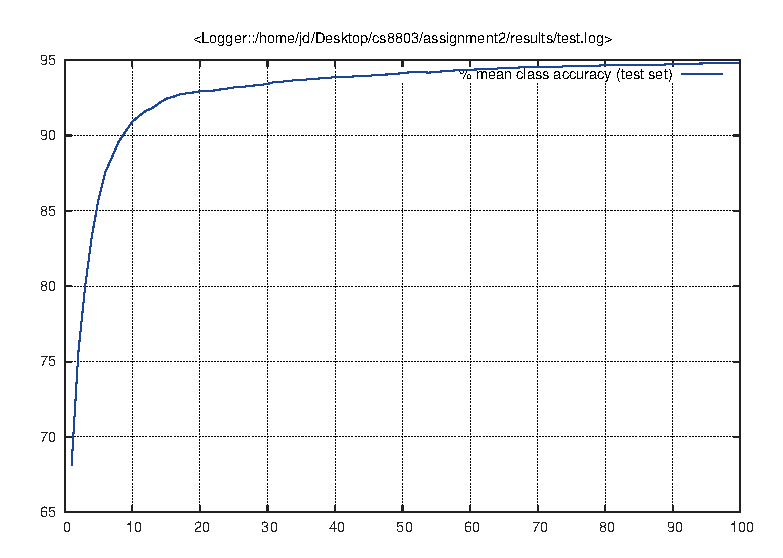
\includegraphics[width=\imsize]{assignment2/results/sgd_test}

Learning rate = 1e-2

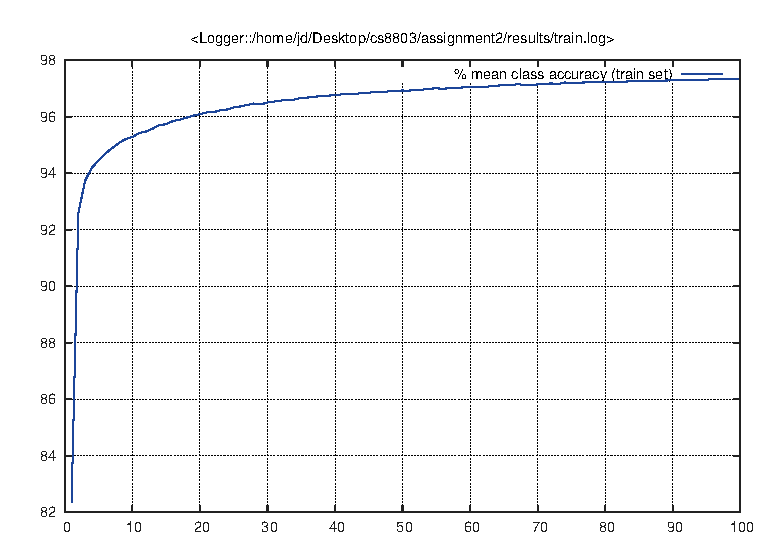
\includegraphics[width=\imsize]{assignment2/results/sgd_r2_train}
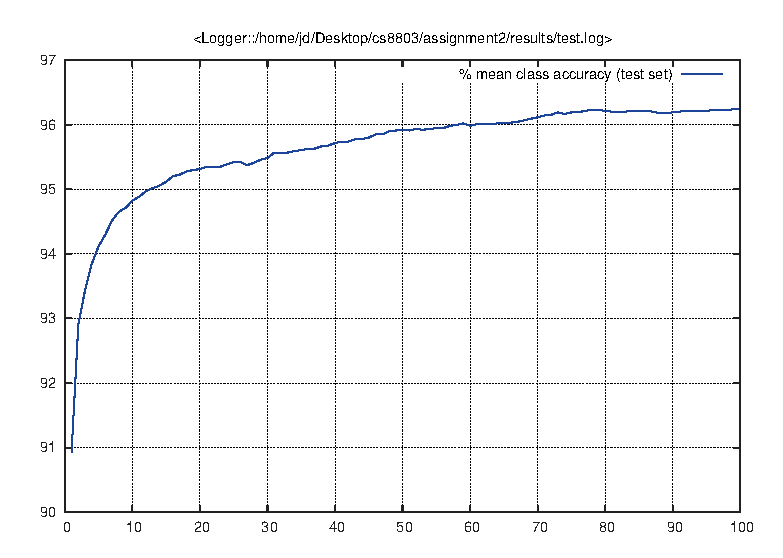
\includegraphics[width=\imsize]{assignment2/results/sgd_r2_test}

Learning rate = 1e-4

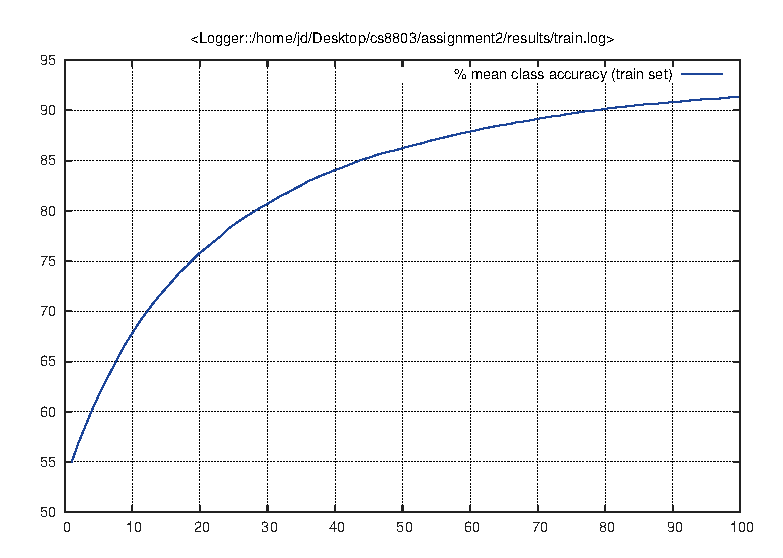
\includegraphics[width=\imsize]{assignment2/results/sgd_r4_train}
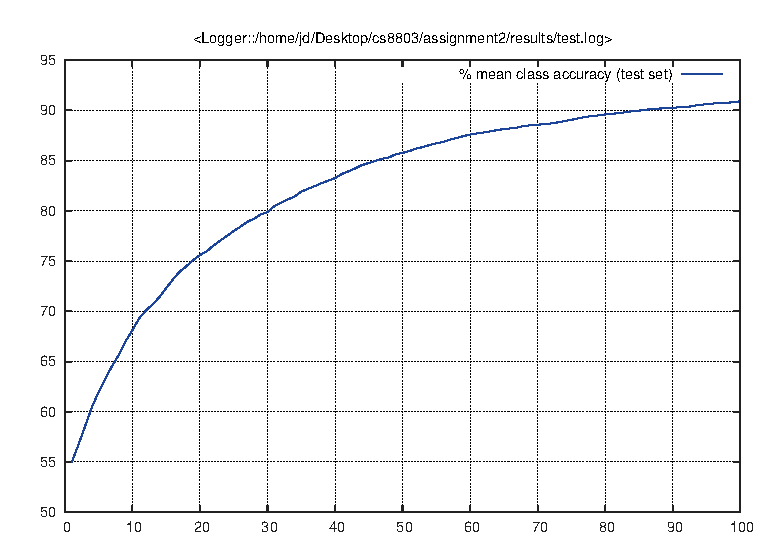
\includegraphics[width=\imsize]{assignment2/results/sgd_r4_test}
Learning rate decay = 1e-5

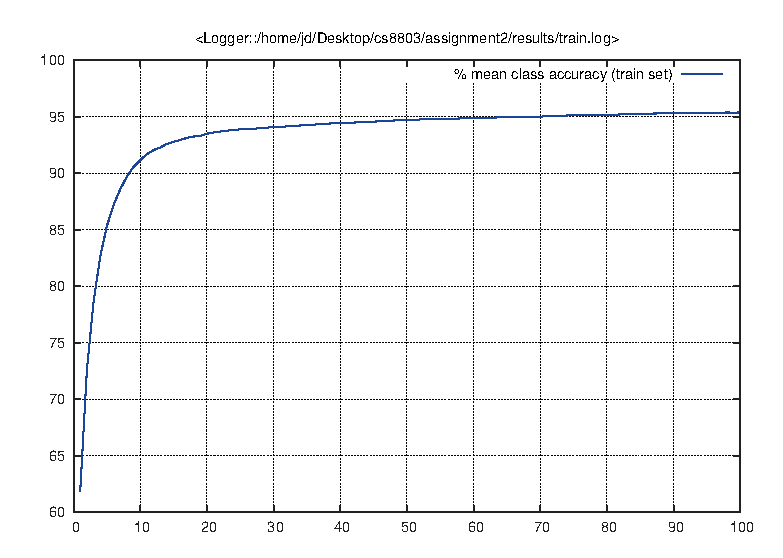
\includegraphics[width=\imsize]{assignment2/results/sgd_d5_train}
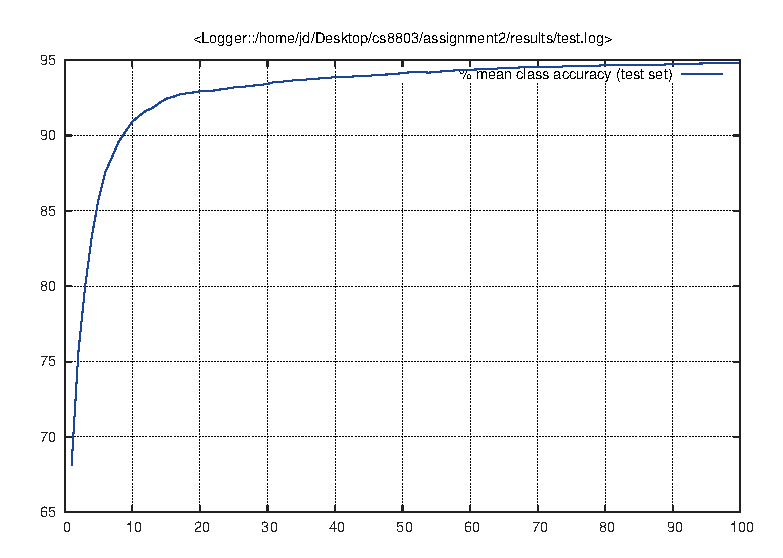
\includegraphics[width=\imsize]{assignment2/results/sgd_d5_test}

Learning rate decay = 1e-6

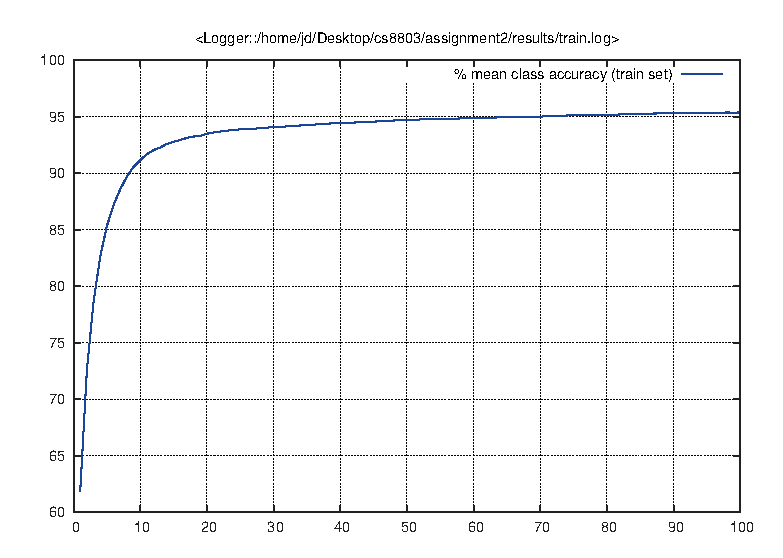
\includegraphics[width=\imsize]{assignment2/results/sgd_d6_train}
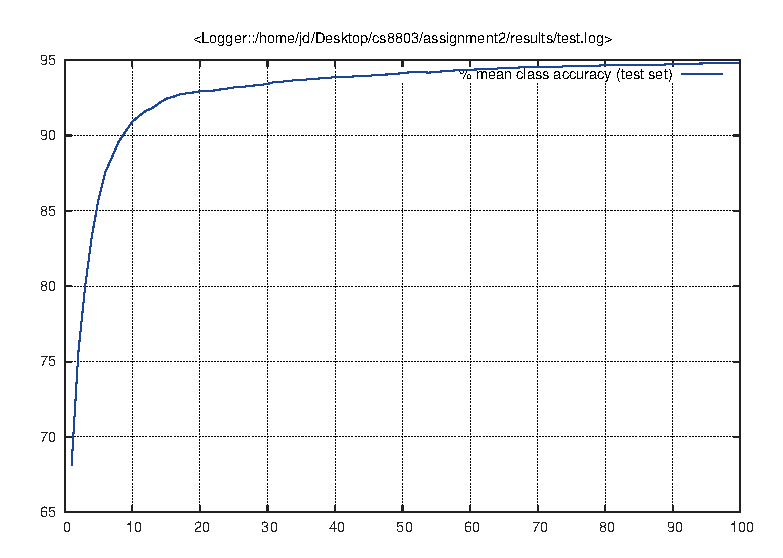
\includegraphics[width=\imsize]{assignment2/results/sgd_d6_test}

\subsection{SGD + weight decay}

Weight decay = 1e-5

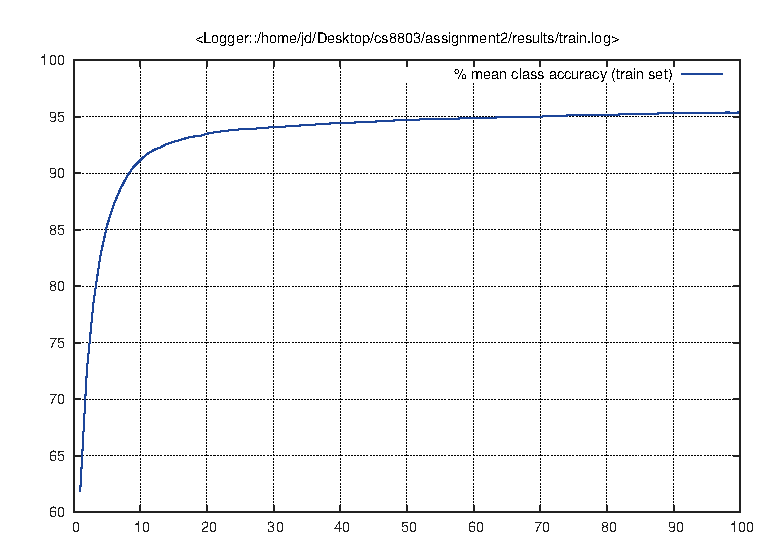
\includegraphics[width=\imsize]{assignment2/results/sgdw_train}
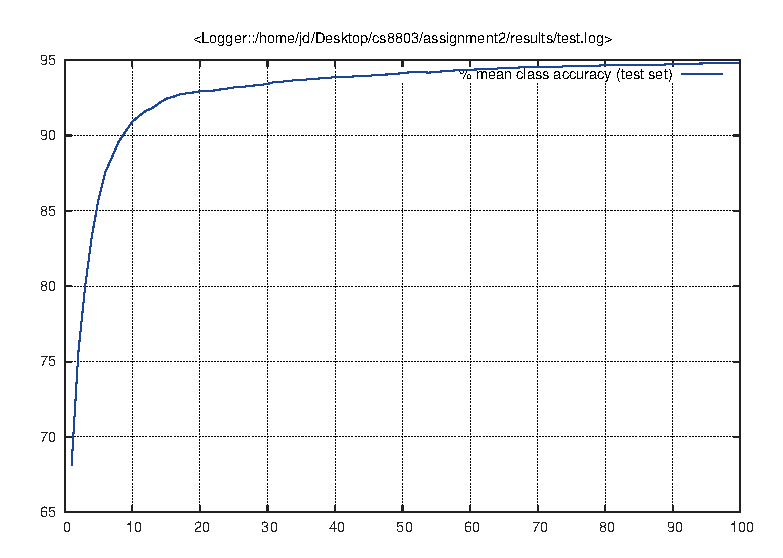
\includegraphics[width=\imsize]{assignment2/results/sgdw_test}

Weight decay = 1e-3

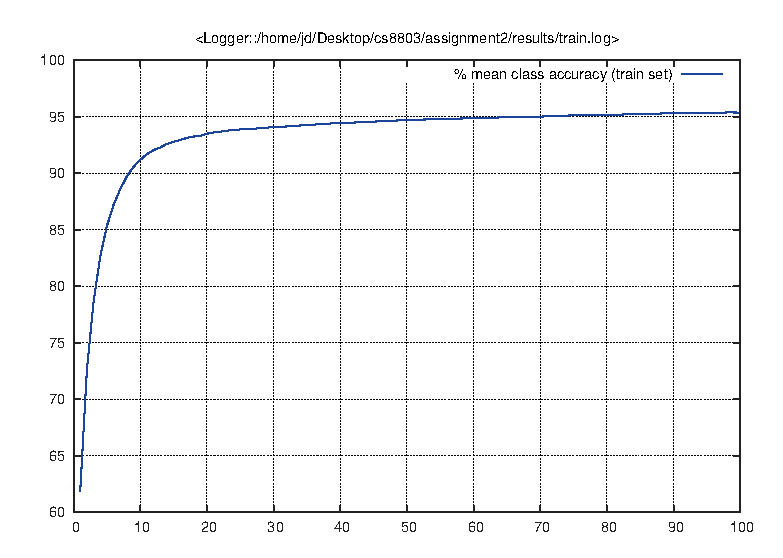
\includegraphics[width=\imsize]{assignment2/results/sgdw_w3_train}
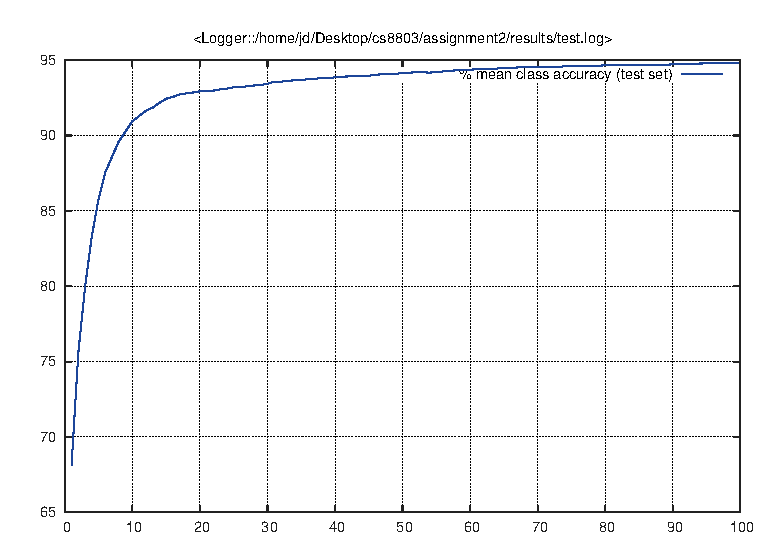
\includegraphics[width=\imsize]{assignment2/results/sgdw_w3_test}

Weight decay = 1e-4

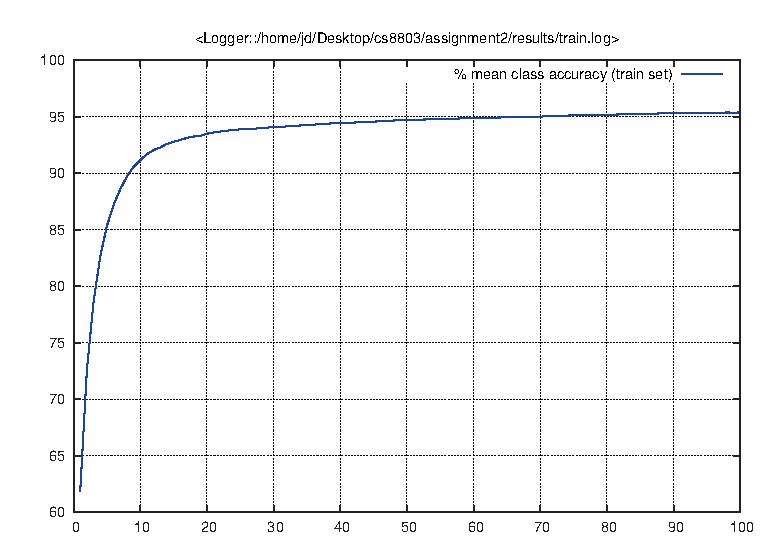
\includegraphics[width=\imsize]{assignment2/results/sgdw_w4_train}
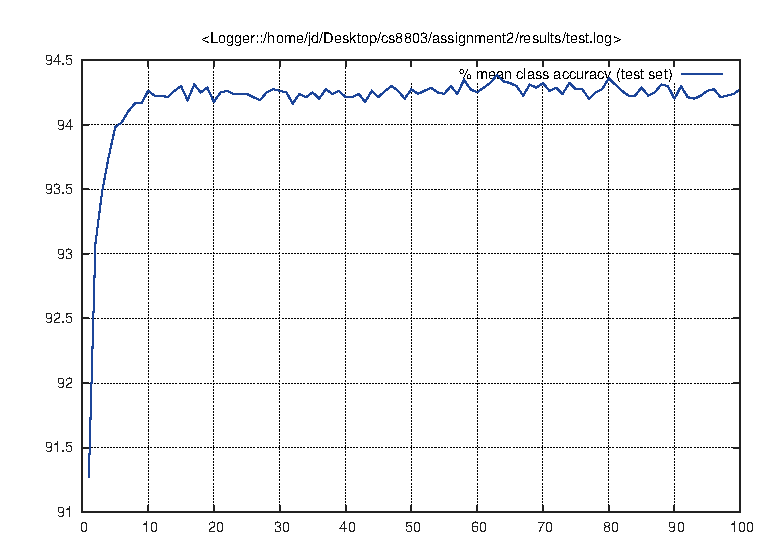
\includegraphics[width=\imsize]{assignment2/results/sgdw_w4_test}

\subsection{SGD + weight decay + momentum}

Momentum = 0.1

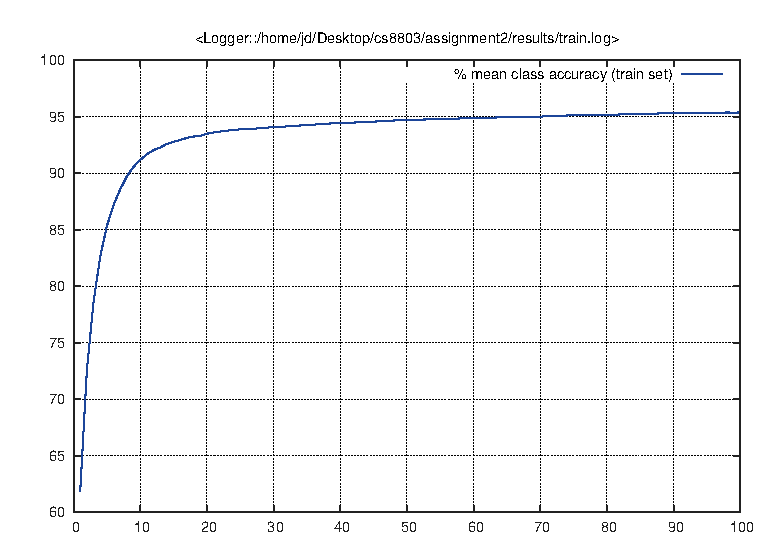
\includegraphics[width=\imsize]{assignment2/results/sgdwm_train}
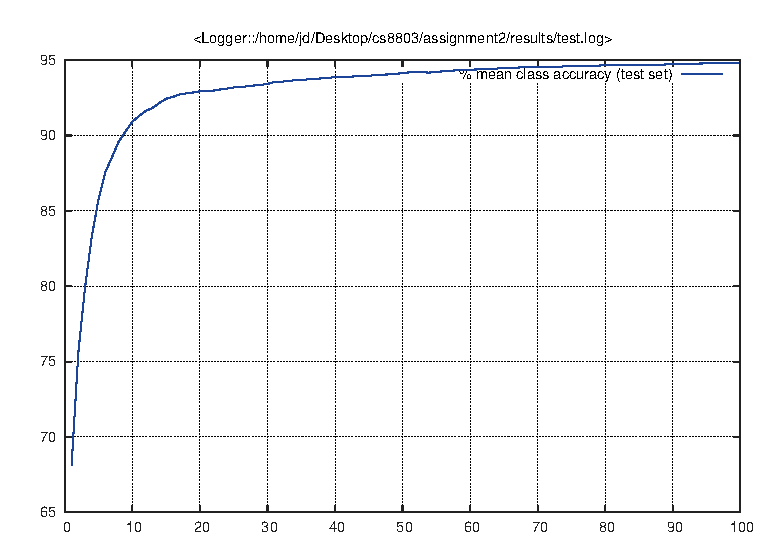
\includegraphics[width=\imsize]{assignment2/results/sgdwm_test}

Momentum = 0.5

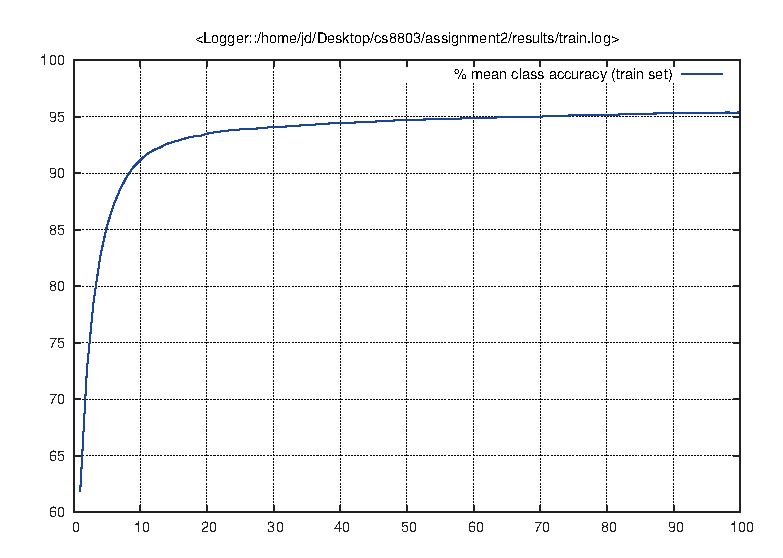
\includegraphics[width=\imsize]{assignment2/results/sgdwm_m5_train}
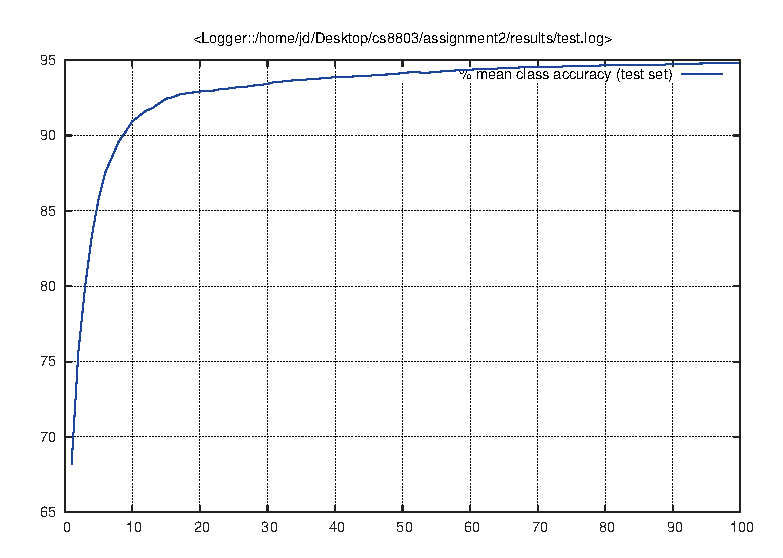
\includegraphics[width=\imsize]{assignment2/results/sgdwm_m5_test}

Momentum = 0.9

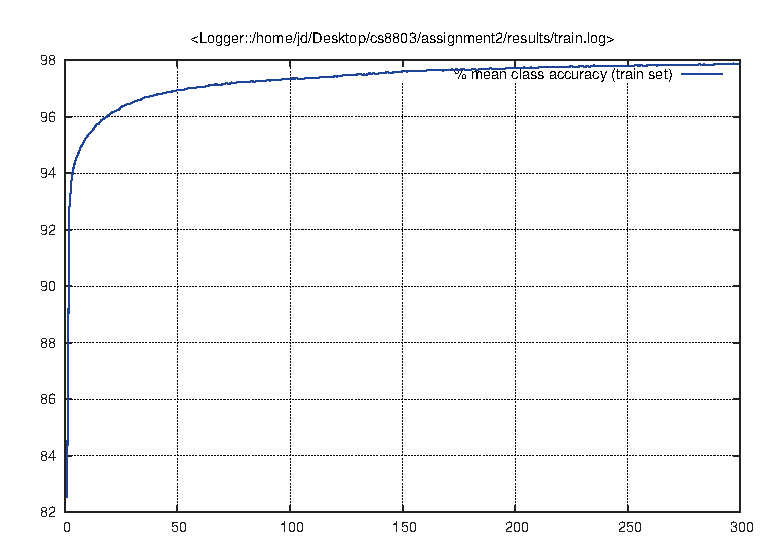
\includegraphics[width=\imsize]{assignment2/results/sgdwm_m9_train}
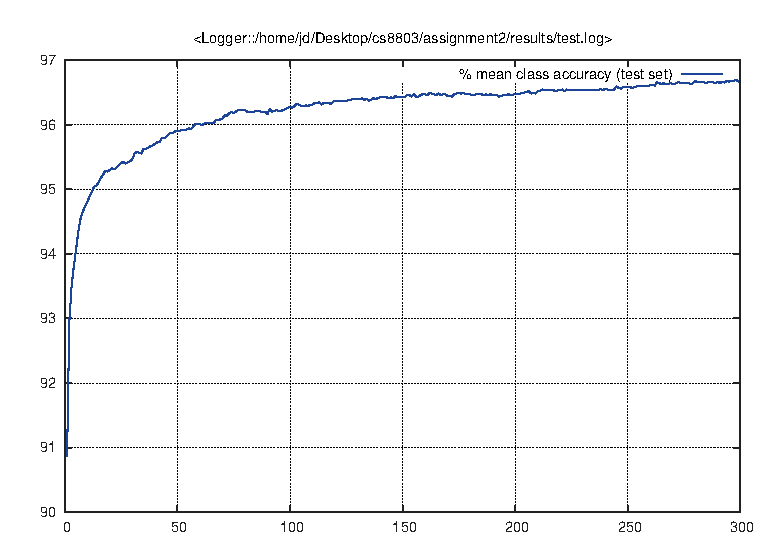
\includegraphics[width=\imsize]{assignment2/results/sgdwm_m9_test}

\subsection{Coordinate Descent}

Learning rate = 1e-4

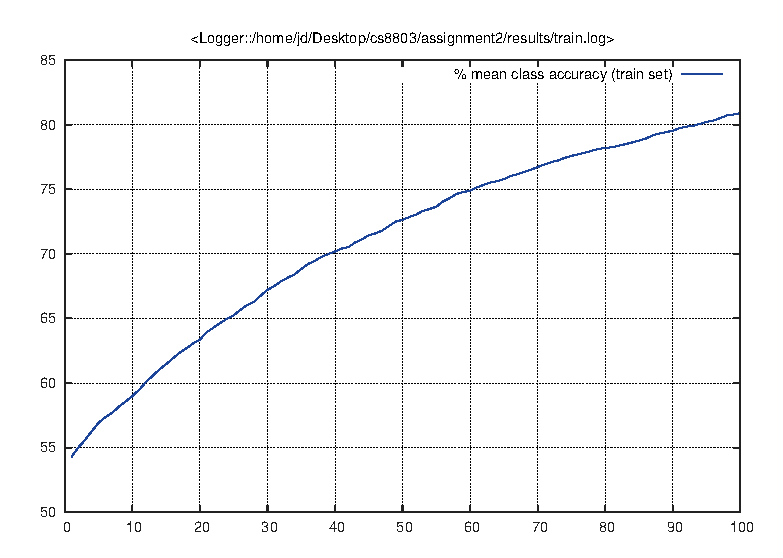
\includegraphics[width=\imsize]{assignment2/results/cd_train}
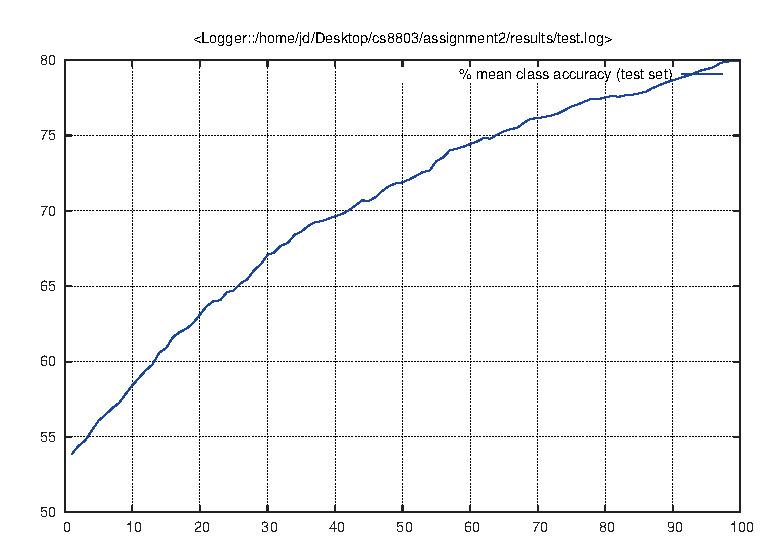
\includegraphics[width=\imsize]{assignment2/results/cd_test}

Learning rate = 1e-3

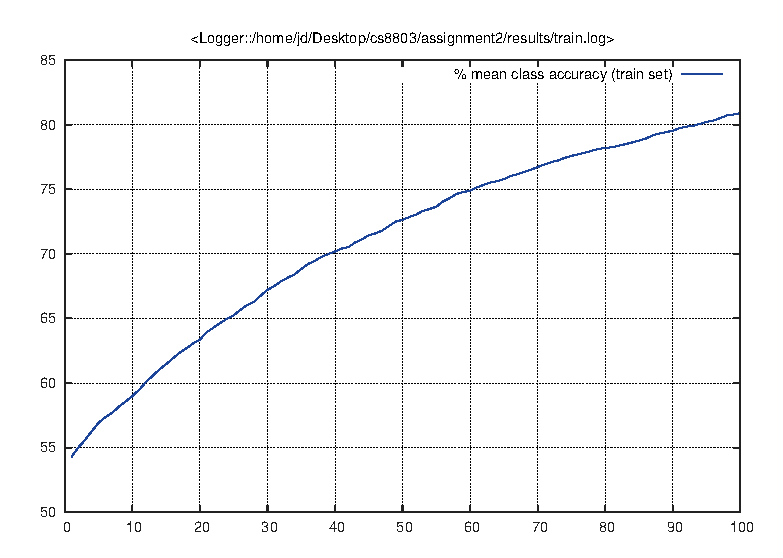
\includegraphics[width=\imsize]{assignment2/results/cd_lr3_train}
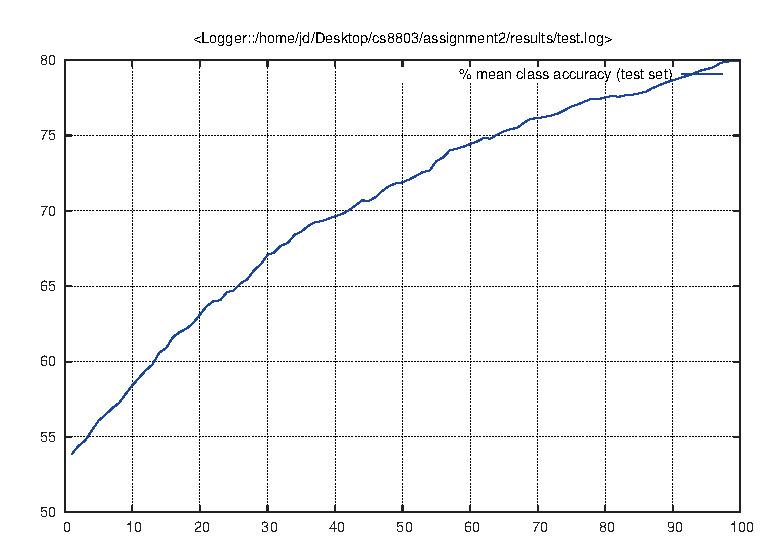
\includegraphics[width=\imsize]{assignment2/results/cd_lr3_test}

Learning rate = 1e-5

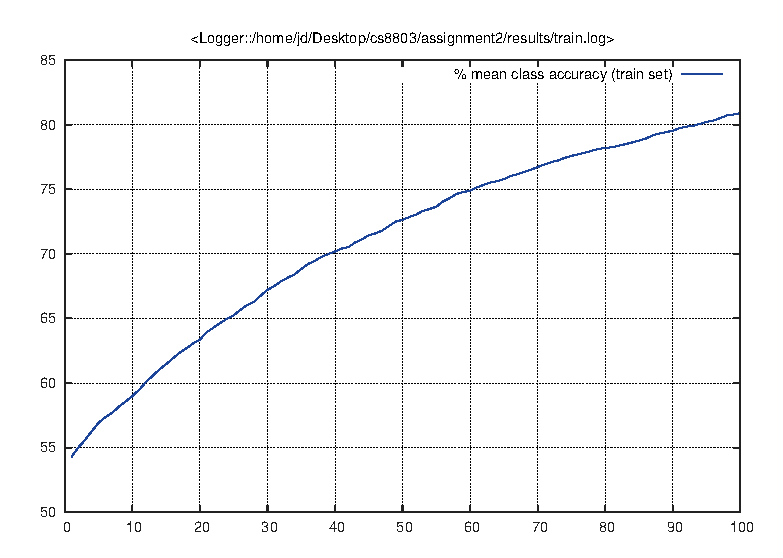
\includegraphics[width=\imsize]{assignment2/results/cd_lr5_train}
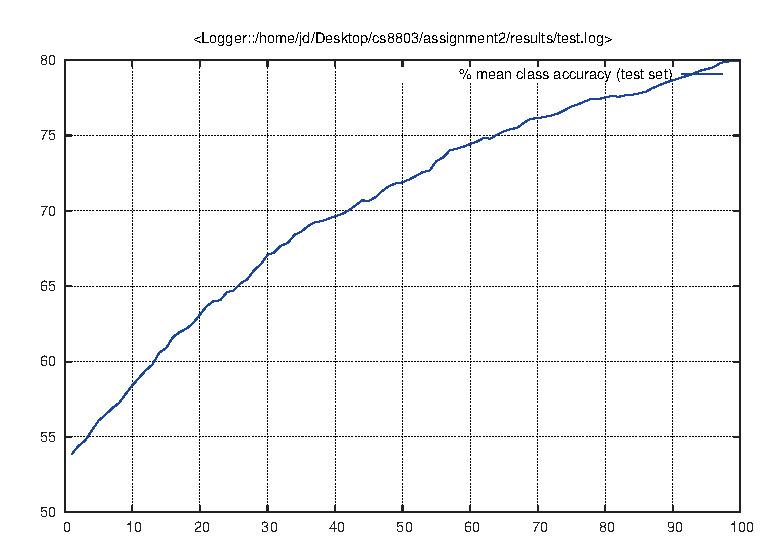
\includegraphics[width=\imsize]{assignment2/results/cd_lr5_test}

\subsection{Analysis}

The above tests were conducted over 100 epochs with different gradient descent methods.
Each method differed in terms of convergence rate with respect to their parameters.
For basic stochastic gradient descent, an increase in learning rate increases convergence rate
but leads to more oscillation, whereas learning rate decay causes convergence to slow down
for later iterations. 

\section{Activation}
The plots of training and test error for each method is shown below:

\subsection{Tanh}
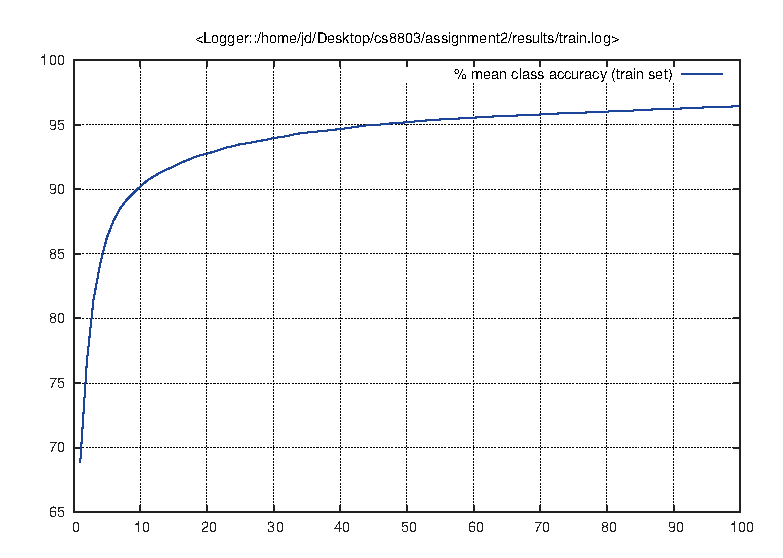
\includegraphics[width=\imsize]{assignment2/results/tanh_train}
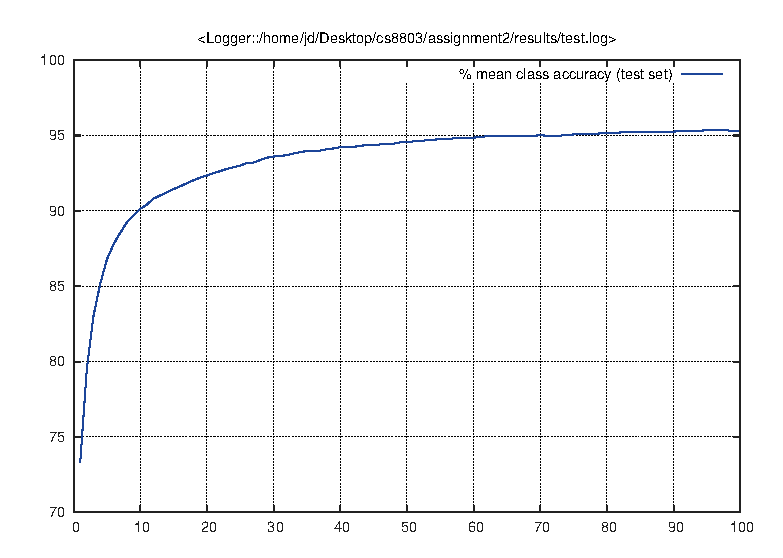
\includegraphics[width=\imsize]{assignment2/results/tanh_test}
\subsection{Sigmoid}
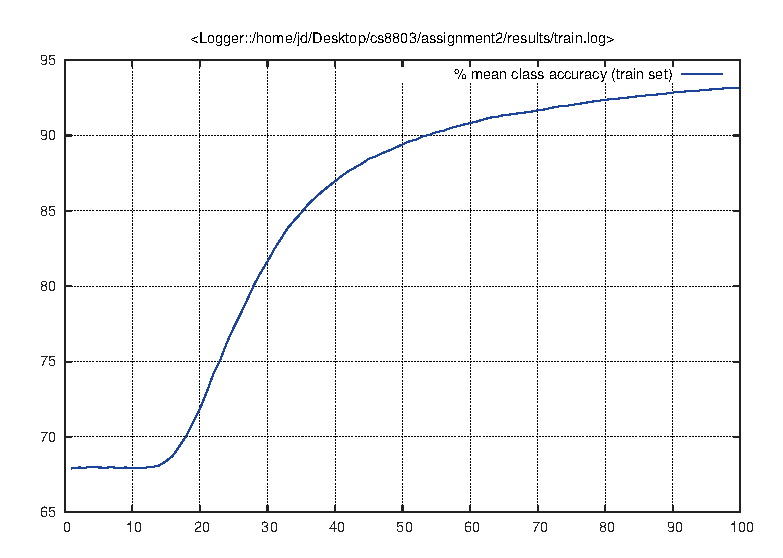
\includegraphics[width=\imsize]{assignment2/results/sigmoid_train}
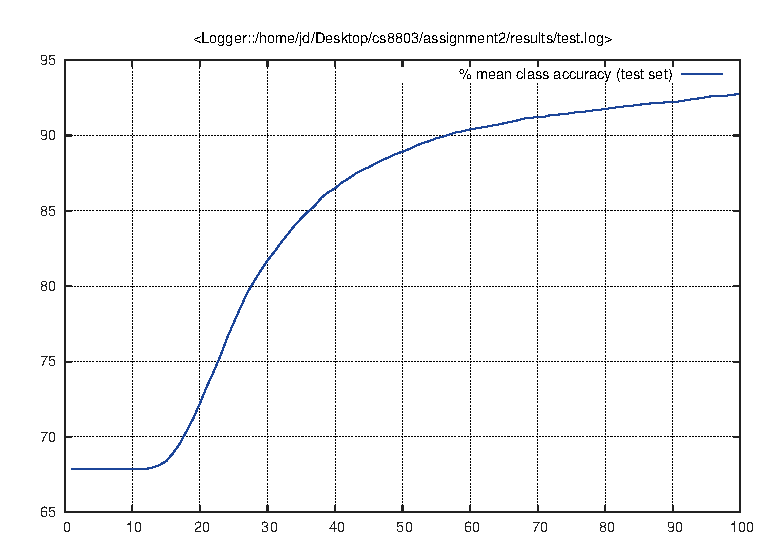
\includegraphics[width=\imsize]{assignment2/results/sigmoid_test}
\subsection{Rectified Linear Unit}
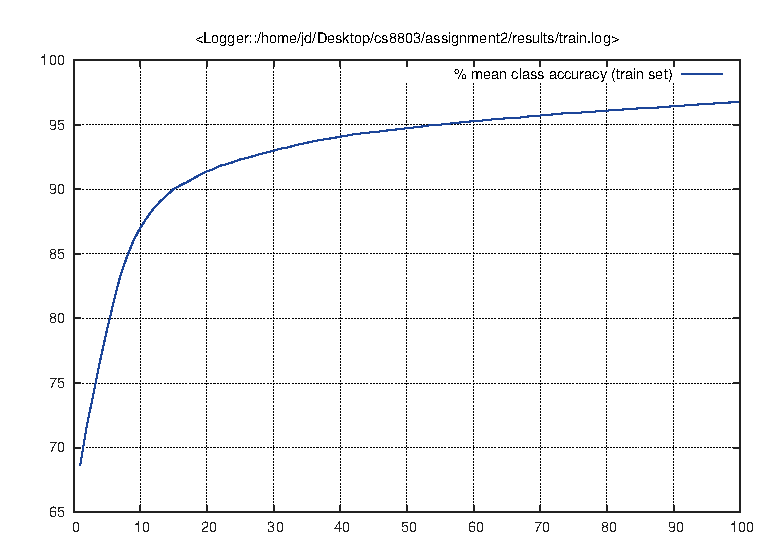
\includegraphics[width=\imsize]{assignment2/results/relu_train}
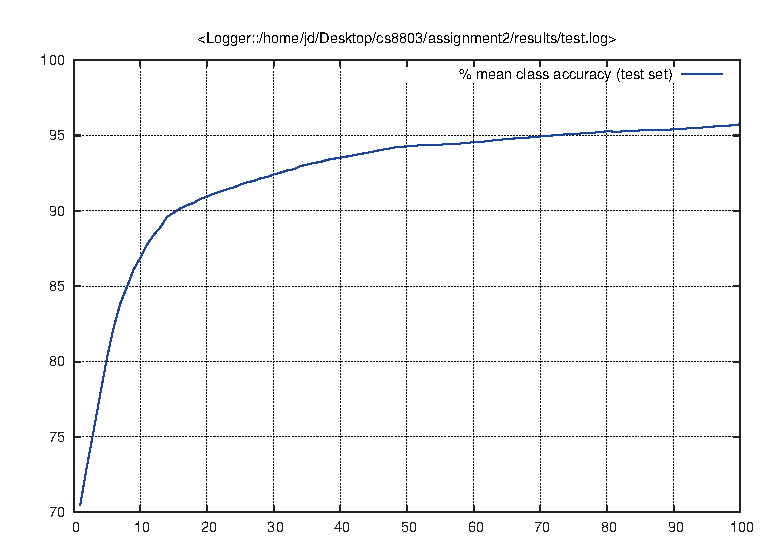
\includegraphics[width=\imsize]{assignment2/results/relu_test}
\subsection{Rectified Quadratic Unit}
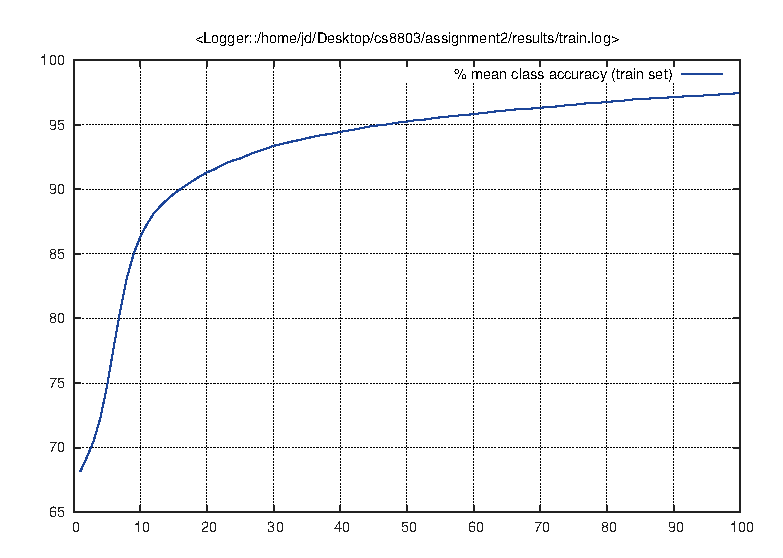
\includegraphics[width=\imsize]{assignment2/results/requ_train}
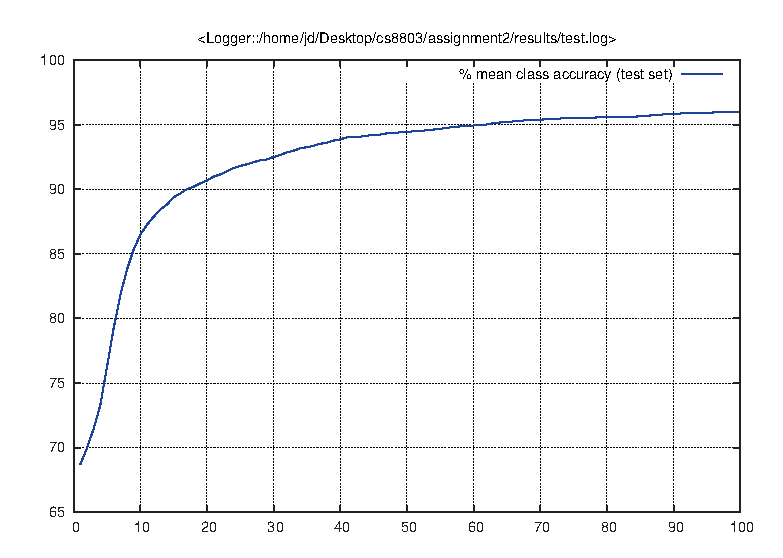
\includegraphics[width=\imsize]{assignment2/results/requ_test}

\subsection{Comparison}

From the plots of training and test error, tanh showed fast convergence rate whereas sigmoid demonstrated
slow convergence at earlier iterations. The Rectified Linear and Quadratic Unit also showed slightly faster
convergence rate compared to tanh. A major difference between sigmoid (or tanh) and ReLU (ReQU) is that
the former plateaus at later iterations whereas the latter continues to improve.

\end{document}
